\documentclass[aspectratio=169]{beamer}
\usepackage{amsmath}
\usepackage{amssymb}
\usepackage{graphicx}
\usepackage{tcolorbox}
\usepackage{booktabs}
\usepackage{colortbl}
\usepackage{xcolor}
\usepackage{tikz}
\usetikzlibrary{angles,quotes}
\usepackage[utf8]{inputenc}

% Custom colors
\definecolor{primary}{RGB}{41, 128, 185}
\definecolor{secondary}{RGB}{52, 152, 219}
\definecolor{accent}{RGB}{231, 76, 60}
\definecolor{lightgray}{RGB}{236, 240, 241}

% Theme customization
\usetheme{Madrid}
\usecolortheme{whale}
\setbeamercolor{structure}{fg=primary}
\setbeamercolor{background canvas}{bg=white}
\setbeamercolor{normal text}{fg=black}

% Title page info
\title{Pre-Calculus 11}
\subtitle{Basic Trigonometric Functions}
\author{Created by Yi-Chen Lin}
\date{\today}

\begin{document}

\begin{frame}
    \titlepage
\end{frame}

% I) WHAT IS TRIGONOMETRY?
\begin{frame}{What is Trigonometry?}
    \begin{tcolorbox}[colback=lightgray,colframe=primary,title=Introduction]
        \footnotesize
        \begin{columns}
            \column{0.6\textwidth}
            \begin{itemize}
                \item Study of the relationship between the angles in a right triangle with the lengths of the sides
                \item Basic trigonometry deals mainly with Right Triangles
                \item There are three basic trigonometry functions:
                \begin{itemize}
                    \item Sine, Cosine, and Tangent [look for them on your calculator]
                \end{itemize}
                \item These trig. Functions will give you the ratios of the sides in a right triangle
            \end{itemize}
            \column{0.4\textwidth}
            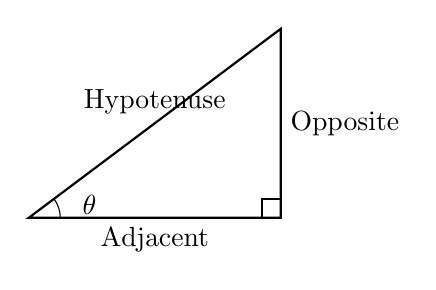
\begin{tikzpicture}[scale=0.8]
                \draw[thick] (0,0) -- (4,0) -- (4,3) -- cycle;
                \draw[thick] (3.7,0) -- (3.7,0.3) -- (4,0.3);
                \node[right] at (4,1.5) {Opposite};
                \node[below] at (2,0) {Adjacent};
                \node[above, sloped] at (2,1.5) {Hypotenuse};
                \draw (0.5,0) arc (0:36.87:0.5);
                \node[right] at (0.7,0.2) {$\theta$};
            \end{tikzpicture}
        \end{columns}
    \end{tcolorbox}
\end{frame}

\begin{frame}{Basic Trig Ratios}
    \begin{tcolorbox}[colback=lightgray,colframe=accent,title=Example]
        \footnotesize
        \begin{columns}
            \column{0.6\textwidth}
            For a right triangle with angle 22.62°:
            \begin{align*}
                \sin 22.62^\circ &= \frac{5}{13} \approx 0.38461538... \\
                \cos 22.62^\circ &= \frac{12}{13} \approx 0.92307692... \\
                \tan 22.62^\circ &= \frac{5}{12} \approx 0.41666666...
            \end{align*}
            \column{0.4\textwidth}
            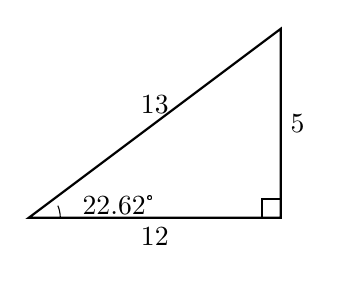
\begin{tikzpicture}[scale=0.8]
                \draw[thick] (0,0) -- (4,0) -- (4,3) -- cycle;
                \draw[thick] (3.7,0) -- (3.7,0.3) -- (4,0.3);
                \node[right] at (4,1.5) {5};
                \node[below] at (2,0) {12};
                \node[above, sloped] at (2,1.5) {13};
                \draw (0.5,0) arc (0:22.62:0.5); % Changed to 22.62
                \node[right] at (0.7,0.2) {22.62°};
            \end{tikzpicture}
        \end{columns}
    \end{tcolorbox}
\end{frame}

% II) NAMING SIDES OF A RIGHT TRIANGLE
\begin{frame}{Naming Sides of a Right Triangle}
    \begin{tcolorbox}[colback=lightgray,colframe=primary,title=Important Notes]
        \footnotesize
        \begin{columns}
            \column{0.6\textwidth}
            \begin{itemize}
                \item When naming the sides of a R.T., they are relative to the angle that you are using
                \item The Adjacent and Opposite side can be switched around depending on which angle you use
                \item The Hypotenuse must be the longest side and opposite from the "box"
                \item When using Trig, make sure your calculator is on "DEG" mode
            \end{itemize}
            \column{0.4\textwidth}
            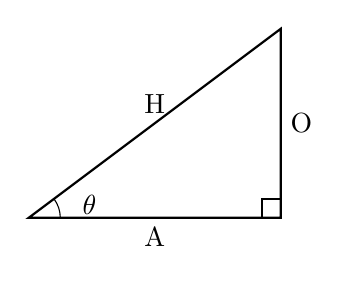
\begin{tikzpicture}[scale=0.8]
                \draw[thick] (0,0) -- (4,0) -- (4,3) -- cycle;
                \draw[thick] (3.7,0) -- (3.7,0.3) -- (4,0.3);
                \node[right] at (4,1.5) {O};
                \node[below] at (2,0) {A};
                \node[above, sloped] at (2,1.5) {H};
                \draw (0.5,0) arc (0:36.87:0.5);
                \node[right] at (0.7,0.2) {$\theta$};
            \end{tikzpicture}
        \end{columns}
    \end{tcolorbox}
\end{frame}

% III) SOH-CAH-TOA
\begin{frame}{SOH-CAH-TOA}
    \begin{tcolorbox}[colback=lightgray,colframe=accent,title=Trigonometric Ratios]
        \footnotesize
        \begin{columns}
            \column{0.6\textwidth}
            \begin{align*}
                \sin \theta &= \frac{\text{Opposite}}{\text{Hypotenuse}} \\
                \cos \theta &= \frac{\text{Adjacent}}{\text{Hypotenuse}} \\
                \tan \theta &= \frac{\text{Opposite}}{\text{Adjacent}}
            \end{align*}
            \begin{itemize}
                \item Use SINE when working with Opposite or Hypotenuse
                \item Use COSINE when working with Adjacent or Hypotenuse
                \item Use TANGENT when working with Opposite or Adjacent
            \end{itemize}
            \column{0.4\textwidth}
            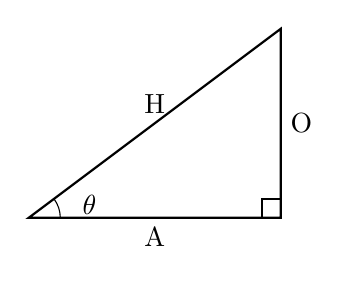
\begin{tikzpicture}[scale=0.8]
                \draw[thick] (0,0) -- (4,0) -- (4,3) -- cycle;
                \draw[thick] (3.7,0) -- (3.7,0.3) -- (4,0.3);
                \node[right] at (4,1.5) {O};
                \node[below] at (2,0) {A};
                \node[above, sloped] at (2,1.5) {H};
                \draw (0.5,0) arc (0:36.87:0.5);
                \node[right] at (0.7,0.2) {$\theta$};
            \end{tikzpicture}
        \end{columns}
    \end{tcolorbox}
\end{frame}

% IV) FINDING MISSING SIDES
\begin{frame}{Finding Missing Sides}
    \begin{tcolorbox}[colback=lightgray,colframe=primary,title=Steps to Find Missing Sides]
        \footnotesize
        \begin{columns}
            \column{0.6\textwidth}
            \begin{enumerate}
                \item Identify which sides are given (name them based on the angle)
                \item Determine which trig function to use: SOH - CAH - TOA
                \item Write the equation and use algebra to find the missing side
                \item Make sure your calculator is in DEG mode!
            \end{enumerate}
            \column{0.4\textwidth}
            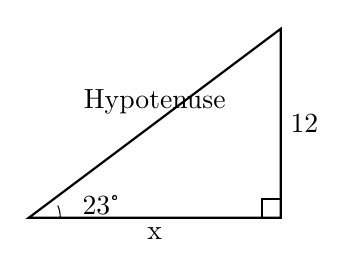
\begin{tikzpicture}[scale=0.8]
                \draw[thick] (0,0) -- (4,0) -- (4,3) -- cycle;
                \draw[thick] (3.7,0) -- (3.7,0.3) -- (4,0.3);
                \node[right] at (4,1.5) {12};
                \node[below] at (2,0) {x};
                \node[above, sloped] at (2,1.5) {Hypotenuse};
                \draw (0.5,0) arc (0:23:0.5);
                \node[right] at (0.7,0.2) {23°};
            \end{tikzpicture}
        \end{columns}
    \end{tcolorbox}
\end{frame}

\begin{frame}{Example: Finding Missing Side}
    \begin{tcolorbox}[colback=lightgray,colframe=accent,title=Example]
        \footnotesize
        \begin{columns}
            \column{0.6\textwidth}
            Find x:
            \begin{align*}
                \tan 23^\circ &= \frac{12}{x} \\
                0.4244748162 &= \frac{12}{x} \\
                x &= \frac{12}{0.4244748162} \\
                x &\approx 28.2702
            \end{align*}
            \column{0.4\textwidth}
            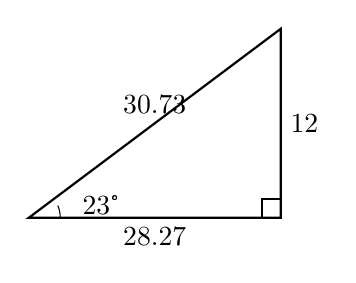
\begin{tikzpicture}[scale=0.8]
                \draw[thick] (0,0) -- (4,0) -- (4,3) -- cycle;
                \draw[thick] (3.7,0) -- (3.7,0.3) -- (4,0.3);
                \node[right] at (4,1.5) {12};
                \node[below] at (2,0) {28.27};
                \node[above, sloped] at (2,1.5) {30.73};
                \draw (0.5,0) arc (0:23:0.5); % Corrected angle
                \node[right] at (0.7,0.2) {23°};
            \end{tikzpicture}
        \end{columns}
    \end{tcolorbox}
\end{frame}

% V) USING TRIG TO FIND MISSING ANGLES
\begin{frame}{Finding Missing Angles}
    \begin{tcolorbox}[colback=lightgray,colframe=primary,title=Important Notes]
        \footnotesize
        \begin{columns}
            \column{0.6\textwidth}
            \begin{itemize}
                \item Use inverse trig functions: $\sin^{-1}$, $\cos^{-1}$, $\tan^{-1}$
                \item First determine which sides are given and which trig function to use
                \item Keep at least 3-4 decimal places for your angles
                \item You can only "Inverse Tan" a ratio, it gives you the angle
            \end{itemize}
            \column{0.4\textwidth}
            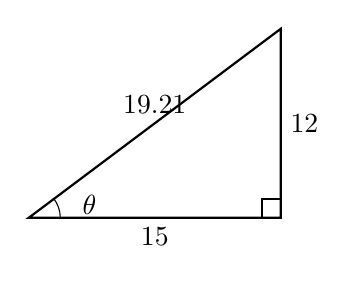
\begin{tikzpicture}[scale=0.8]
                \draw[thick] (0,0) -- (4,0) -- (4,3) -- cycle;
                \draw[thick] (3.7,0) -- (3.7,0.3) -- (4,0.3);
                \node[right] at (4,1.5) {12};
                \node[below] at (2,0) {15};
                \node[above, sloped] at (2,1.5) {19.21};
                \draw (0.5,0) arc (0:38.66:0.5); % Corrected angle to match ratio
                \node[right] at (0.7,0.2) {$\theta$};
            \end{tikzpicture}
        \end{columns}
    \end{tcolorbox}
\end{frame}

\begin{frame}{Example: Finding Missing Angle}
    \begin{tcolorbox}[colback=lightgray,colframe=accent,title=Example]
        \footnotesize
        \begin{columns}
            \column{0.6\textwidth}
            Find $\theta$:
            \begin{align*}
                \tan \theta &= \frac{12}{15} \\
                \theta &= \tan^{-1}\left(\frac{12}{15}\right) \\
                \theta &\approx 38.6598^\circ
            \end{align*}
            \column{0.4\textwidth}
            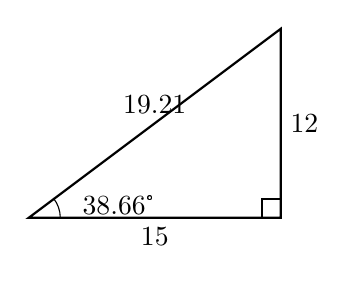
\begin{tikzpicture}[scale=0.8]
                \draw[thick] (0,0) -- (4,0) -- (4,3) -- cycle;
                \draw[thick] (3.7,0) -- (3.7,0.3) -- (4,0.3);
                \node[right] at (4,1.5) {12};
                \node[below] at (2,0) {15};
                \node[above, sloped] at (2,1.5) {19.21};
                \draw (0.5,0) arc (0:38.66:0.5);
                \node[right] at (0.7,0.2) {38.66°};
            \end{tikzpicture}
        \end{columns}
    \end{tcolorbox}
\end{frame}

% Practice: Identify sides and trig function
\begin{frame}{Practice: Identify Sides & Trig Function - Part 1}
    \begin{tcolorbox}[colback=lightgray,colframe=primary,title=Indicate Sides (Opp, Adj, Hyp) and Trig Function]
        \footnotesize
        Indicate which sides are given: Opp, Adj, or Hyp. Then indicate which trig function should be used to solve the triangle.\\
        \vspace{0.5em}
        \begin{columns}
            \column{0.33\textwidth}
                a)
                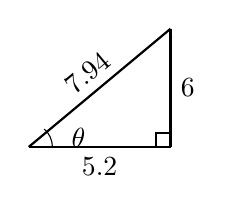
\begin{tikzpicture}[scale=0.6]
                    \draw[thick] (0,0) -- (3,0) node[below, pos=0.5] {5.2};
                    \draw[thick] (3,0) -- (3,2.5) node[right, pos=0.5] {6};
                    \draw[thick] (3,2.5) -- (0,0) node[above, sloped, pos=0.5] {7.94}; % Hypotenuse
                    \draw[thick] (2.7,0) -- (2.7,0.3) -- (3,0.3); % Right angle
                    \draw (0.5,0) arc (0:49.07:0.5); % Angle theta
                    \node[right] at (0.7,0.2) {$\theta$};
                \end{tikzpicture}
            \column{0.33\textwidth}
                b)
                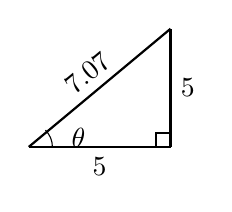
\begin{tikzpicture}[scale=0.6]
                    \draw[thick] (0,0) -- (3,0) node[below, pos=0.5] {5};
                    \draw[thick] (3,0) -- (3,2.5) node[right, pos=0.5] {5};
                    \draw[thick] (3,2.5) -- (0,0) node[above, sloped, pos=0.5] {7.07}; % Hypotenuse
                    \draw[thick] (2.7,0) -- (2.7,0.3) -- (3,0.3); % Right angle
                    \draw (0.5,0) arc (0:45:0.5); % Angle theta at (0,0)
                    \node[right] at (0.7,0.2) {$\theta$};
                \end{tikzpicture}
            \column{0.33\textwidth}
                c)
                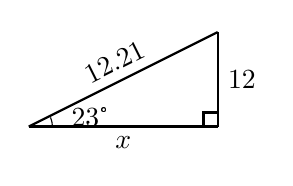
\begin{tikzpicture}[scale=0.6]
                    \draw[thick] (0,0) -- (4,0) node[below, pos=0.5] {$x$};
                    \draw[thick] (4,0) -- (4,2) node[right, pos=0.5] {12};
                    \draw[thick] (4,2) -- (0,0) node[above, sloped, pos=0.5] {12.21}; % Hypotenuse (calculated from previous value)
                    \draw[thick] (3.7,0) -- (3.7,0.3) -- (4,0.3);
                    \draw (0.5,0) arc (0:23:0.5);
                    \node[right] at (0.7,0.2) {23°};
                \end{tikzpicture}
        \end{columns}
    \end{tcolorbox}
\end{frame}

\begin{frame}{Practice: Identify Sides & Trig Function - Part 2}
    \begin{tcolorbox}[colback=lightgray,colframe=primary,title=Indicate Sides (Opp, Adj, Hyp) and Trig Function]
        \footnotesize
        Indicate which sides are given: Opp, Adj, or Hyp. Then indicate which trig function should be used to solve the triangle.\\
        \vspace{1em}
        \begin{columns}
            \column{0.33\textwidth}
                d)
                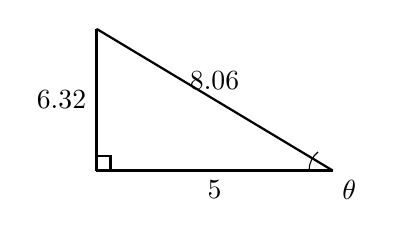
\begin{tikzpicture}[scale=0.6]
                    % Vertices (0,0), (5,0), (0,3)
                    \draw[thick] (0,0) -- (5,0) node[below] at (2.5,0) {5};
                    \draw[thick] (0,0) -- (0,3) node[left] at (0,1.5) {6.32}; % Vertical side
                    \draw[thick] (5,0) -- (0,3) node[above, sloped] at (2.5,1.5) {8.06}; % Hypotenuse
                    \draw[thick] (0.3,0) -- (0.3,0.3) -- (0,0.3); % Right angle at (0,0)
                    % Angle theta at (5,0) - arctan(6.32/5) = 51.78 degrees
                    \draw (5-0.5,0) arc (180:180-51.78:0.5);
                    \node[below right] at (5,0) {$\theta$};
                \end{tikzpicture}
            \column{0.33\textwidth}
                e)
                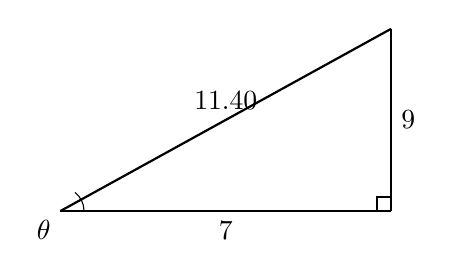
\begin{tikzpicture}[scale=0.6]
                    % Vertices (0,0), (7,0), (7,3.857)
                    \draw[thick] (0,0) -- (7,0) node[below] at (3.5,0) {7};
                    \draw[thick] (7,0) -- (7,3.857) node[right] at (7,1.9285) {9};
                    \draw[thick] (7,3.857) -- (0,0) node[above, sloped] at (3.5,1.9285) {11.40};
                    \draw[thick] (6.7,0) -- (6.7,0.3) -- (7,0.3); % Right angle at (7,0)
                    % Angle theta at (0,0) - arctan(9/7) = 52.12 degrees
                    \draw (0.5,0) arc (0:52.12:0.5);
                    \node[below left] at (0,0) {$\theta$};
                \end{tikzpicture}
            \column{0.33\textwidth}
                f)
                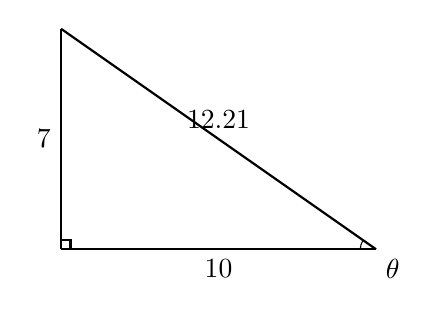
\begin{tikzpicture}[scale=0.4]
                    % Vertices (0,0), (10,0), (0,7)
                    \draw[thick] (0,0) -- (10,0) node[below] at (5,0) {10};
                    \draw[thick] (0,0) -- (0,7) node[left] at (0,3.5) {7}; % Vertical side
                    \draw[thick] (10,0) -- (0,7) node[above, sloped] at (5,3.5) {12.21}; % Hypotenuse
                    \draw[thick] (0.3,0) -- (0.3,0.3) -- (0,0.3); % Right angle at (0,0)
                    % Angle theta at (10,0) - arctan(7/10) = 34.99 degrees
                    \draw (10-0.5,0) arc (180:180-34.99:0.5);
                    \node[below right] at (10,0) {$\theta$};
                \end{tikzpicture}
        \end{columns}
    \end{tcolorbox}
\end{frame}

% Practice: Finding Missing Sides - Part 1
\begin{frame}{Practice: Finding Missing Sides - Part 1}
    \begin{tcolorbox}[colback=lightgray,colframe=accent,title=Find the length of the missing sides]
        \footnotesize
        \begin{columns}
            \column{0.33\textwidth}
                a)
                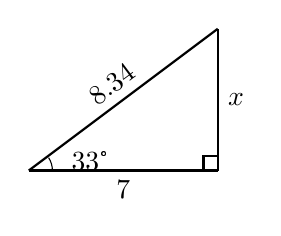
\begin{tikzpicture}[scale=0.6]
                    \draw[thick] (0,0) -- (4,0) node[below, pos=0.5] {7};
                    \draw[thick] (4,0) -- (4,3) node[right, pos=0.5] {$x$};
                    \draw[thick] (4,3) -- (0,0) node[above, sloped, pos=0.5] {8.34}; % Hypotenuse
                    \draw[thick] (3.7,0) -- (3.7,0.3) -- (4,0.3);
                    \draw (0.5,0) arc (0:33:0.5);
                    \node[right] at (0.7,0.2) {33°};
                \end{tikzpicture}
            \column{0.33\textwidth}
                b)
                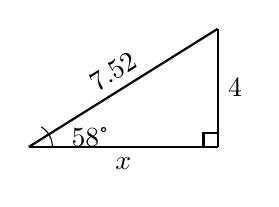
\begin{tikzpicture}[scale=0.6]
                    \draw[thick] (0,0) -- (4,0) node[below, pos=0.5] {$x$};
                    \draw[thick] (4,0) -- (4,2.5) node[right, pos=0.5] {4};
                    \draw[thick] (4,2.5) -- (0,0) node[above, sloped, pos=0.5] {7.52}; % Hypotenuse
                    \draw[thick] (3.7,0) -- (3.7,0.3) -- (4,0.3);
                    \draw (0.5,0) arc (0:58:0.5);
                    \node[right] at (0.7,0.2) {58°};
                \end{tikzpicture}
            \column{0.33\textwidth}
                c)
                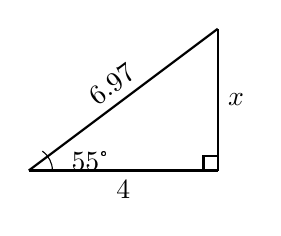
\begin{tikzpicture}[scale=0.6]
                    \draw[thick] (0,0) -- (4,0) node[below, pos=0.5] {4};
                    \draw[thick] (4,0) -- (4,3) node[right, pos=0.5] {$x$};
                    \draw[thick] (4,3) -- (0,0) node[above, sloped, pos=0.5] {6.97}; % Hypotenuse
                    \draw[thick] (3.7,0) -- (3.7,0.3) -- (4,0.3);
                    \draw (0.5,0) arc (0:55:0.5);
                    \node[right] at (0.7,0.2) {55°};
                \end{tikzpicture}
        \end{columns}
    \end{tcolorbox}
\end{frame}

% Practice: Finding Missing Sides - Part 2
\begin{frame}{Practice: Finding Missing Sides - Part 2}
    \begin{tcolorbox}[colback=lightgray,colframe=accent,title=Find the length of the missing sides]
        \footnotesize
        \begin{columns}
            \column{0.33\textwidth}
                d)
                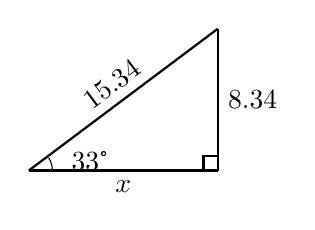
\begin{tikzpicture}[scale=0.6]
                    \draw[thick] (0,0) -- (4,0) node[below, pos=0.5] {$x$};
                    \draw[thick] (4,0) -- (4,3) node[right, pos=0.5] {8.34};
                    \draw[thick] (4,3) -- (0,0) node[above, sloped, pos=0.5] {15.34}; % Hypotenuse
                    \draw[thick] (3.7,0) -- (3.7,0.3) -- (4,0.3);
                    \draw (0.5,0) arc (0:33:0.5);
                    \node[right] at (0.7,0.2) {33°};
                \end{tikzpicture}
            \column{0.33\textwidth}
                e)
                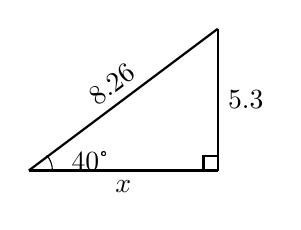
\begin{tikzpicture}[scale=0.6]
                    \draw[thick] (0,0) -- (4,0) node[below, pos=0.5] {$x$};
                    \draw[thick] (4,0) -- (4,3) node[right, pos=0.5] {5.3};
                    \draw[thick] (4,3) -- (0,0) node[above, sloped, pos=0.5] {8.26}; % Hypotenuse
                    \draw[thick] (3.7,0) -- (3.7,0.3) -- (4,0.3);
                    \draw (0.5,0) arc (0:40:0.5);
                    \node[right] at (0.7,0.2) {40°};
                \end{tikzpicture}
            \column{0.33\textwidth}
                f)
                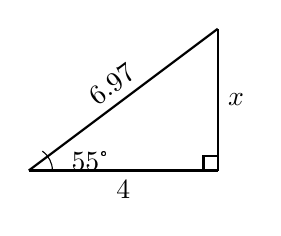
\begin{tikzpicture}[scale=0.6]
                    \draw[thick] (0,0) -- (4,0) node[below, pos=0.5] {4};
                    \draw[thick] (4,0) -- (4,3) node[right, pos=0.5] {$x$};
                    \draw[thick] (4,3) -- (0,0) node[above, sloped, pos=0.5] {6.97}; % Hypotenuse
                    \draw[thick] (3.7,0) -- (3.7,0.3) -- (4,0.3);
                    \draw (0.5,0) arc (0:55:0.5);
                    \node[right] at (0.7,0.2) {55°};
                \end{tikzpicture}
        \end{columns}
    \end{tcolorbox}
\end{frame}

% Practice: Finding Missing Angles - Part 1
\begin{frame}{Practice: Finding Missing Angles - Part 1}
    \begin{tcolorbox}[colback=lightgray,colframe=accent,title=Find the degree of the missing angle]
        \footnotesize
        \begin{columns}
            \column{0.33\textwidth}
                a)
                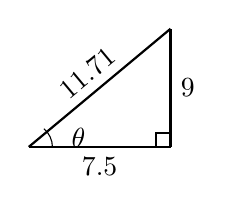
\begin{tikzpicture}[scale=0.6]
                    \draw[thick] (0,0) -- (3,0) node[below, pos=0.5] {7.5};
                    \draw[thick] (3,0) -- (3,2.5) node[right, pos=0.5] {9};
                    \draw[thick] (3,2.5) -- (0,0) node[above, sloped, pos=0.5] {11.71}; % Hypotenuse
                    \draw[thick] (2.7,0) -- (2.7,0.3) -- (3,0.3); % Right angle
                    \draw (0.5,0) arc (0:50.19:0.5); % Calculated angle for tan(theta) = 9/7.5
                    \node[right] at (0.7,0.2) {$\theta$};
                \end{tikzpicture}
            \column{0.33\textwidth}
                b)
                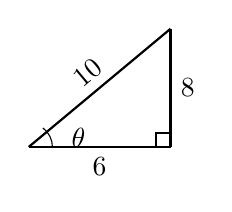
\begin{tikzpicture}[scale=0.6]
                    \draw[thick] (0,0) -- (3,0) node[below, pos=0.5] {6};
                    \draw[thick] (3,0) -- (3,2.5) node[right, pos=0.5] {8};
                    \draw[thick] (3,2.5) -- (0,0) node[above, sloped, pos=0.5] {10}; % Hypotenuse
                    \draw[thick] (2.7,0) -- (2.7,0.3) -- (3,0.3); % Right angle
                    \draw (0.5,0) arc (0:53.13:0.5);
                    \node[right] at (0.7,0.2) {$\theta$};
                \end{tikzpicture}
            \column{0.33\textwidth}
                c)
                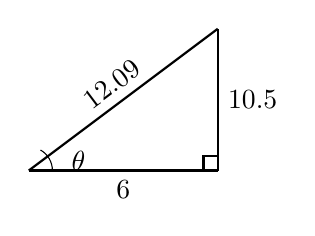
\begin{tikzpicture}[scale=0.6]
                    \draw[thick] (0,0) -- (4,0) node[below, pos=0.5] {6};
                    \draw[thick] (4,0) -- (4,3) node[right, pos=0.5] {10.5};
                    \draw[thick] (4,3) -- (0,0) node[above, sloped, pos=0.5] {12.09}; % Hypotenuse
                    \draw[thick] (3.7,0) -- (3.7,0.3) -- (4,0.3); % Right angle
                    \draw (0.5,0) arc (0:60.25:0.5);
                    \node[right] at (0.7,0.2) {$\theta$};
                \end{tikzpicture}
        \end{columns}
    \end{tcolorbox}
\end{frame}

\begin{frame}{Practice: Finding Missing Angles - Part 2}
    \begin{tcolorbox}[colback=lightgray,colframe=accent,title=Find the degree of the missing angle]
        \footnotesize
        \begin{columns}
            \column{0.33\textwidth}
                d)
                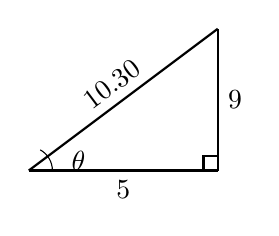
\begin{tikzpicture}[scale=0.6]
                    \draw[thick] (0,0) -- (4,0) node[below, pos=0.5] {5};
                    \draw[thick] (4,0) -- (4,3) node[right, pos=0.5] {9};
                    \draw[thick] (4,3) -- (0,0) node[above, sloped, pos=0.5] {10.30}; % Hypotenuse
                    \draw[thick] (3.7,0) -- (3.7,0.3) -- (4,0.3); % Right angle
                    \draw (0.5,0) arc (0:60.95:0.5);
                    \node[right] at (0.7,0.2) {$\theta$};
                \end{tikzpicture}
            \column{0.33\textwidth}
                e)
                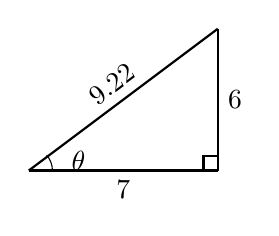
\begin{tikzpicture}[scale=0.6]
                    \draw[thick] (0,0) -- (4,0) node[below, pos=0.5] {7};
                    \draw[thick] (4,0) -- (4,3) node[right, pos=0.5] {6};
                    \draw[thick] (4,3) -- (0,0) node[above, sloped, pos=0.5] {9.22}; % Hypotenuse
                    \draw[thick] (3.7,0) -- (3.7,0.3) -- (4,0.3);
                    \draw (0.5,0) arc (0:40.60:0.5);
                    \node[right] at (0.7,0.2) {$\theta$};
                \end{tikzpicture}
            \column{0.33\textwidth}
                f)
                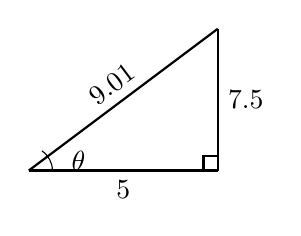
\begin{tikzpicture}[scale=0.6]
                    \draw[thick] (0,0) -- (4,0) node[below, pos=0.5] {5};
                    \draw[thick] (4,0) -- (4,3) node[right, pos=0.5] {7.5};
                    \draw[thick] (4,3) -- (0,0) node[above, sloped, pos=0.5] {9.01}; % Hypotenuse
                    \draw[thick] (3.7,0) -- (3.7,0.3) -- (4,0.3);
                    \draw (0.5,0) arc (0:56.31:0.5);
                    \node[right] at (0.7,0.2) {$\theta$};
                \end{tikzpicture}
        \end{columns}
    \end{tcolorbox}
\end{frame}

% VI) Pythagorean Theorem
\begin{frame}{Pythagorean Theorem}
    \begin{tcolorbox}[colback=lightgray,colframe=primary,title=Pythagorean Theorem]
        \footnotesize
        \begin{columns}
            \column{0.6\textwidth}
            \begin{itemize}
                \item Used to find the missing side lengths of a right triangle when two sides are known.
                \item Formula: $a^2 + b^2 = c^2$, where $a$ and $b$ are the lengths of the two shorter sides (legs), and $c$ is the length of the longest side (hypotenuse).
                \item Also used in trigonometry for fundamental identities like $\sin^2\theta + \cos^2\theta = 1$.
            \end{itemize}
            \column{0.4\textwidth}
            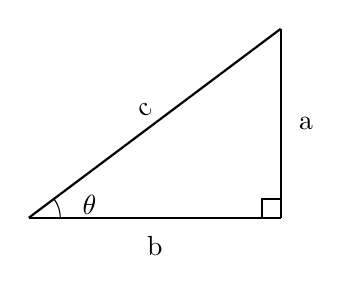
\begin{tikzpicture}[scale=0.8]
                \draw[thick] (0,0) -- (4,0) node[below, pos=0.5, yshift=-0.1cm] {b};
                \draw[thick] (4,0) -- (4,3) node[right, pos=0.5, xshift=0.1cm] {a};
                \draw[thick] (4,3) -- (0,0) node[above, sloped, pos=0.5] {c};
                \draw[thick] (3.7,0) -- (3.7,0.3) -- (4,0.3);
                \draw (0.5,0) arc (0:36.87:0.5);
                \node[right] at (0.7,0.2) {$\theta$};
            \end{tikzpicture}
        \end{columns}
    \end{tcolorbox}
\end{frame}

% VII) Challenge Problem
\begin{frame}{Challenge Problem}
    \begin{tcolorbox}[colback=lightgray,colframe=accent,title=Application of Trigonometry]
        \footnotesize
        \begin{columns}
            \column{0.6\textwidth}
            Two buildings are 70 meters apart. The shorter building is 50m high. A cable is attached to both buildings. The angle of inclination is 15°. How tall is the taller building?
            \column{0.4\textwidth}
            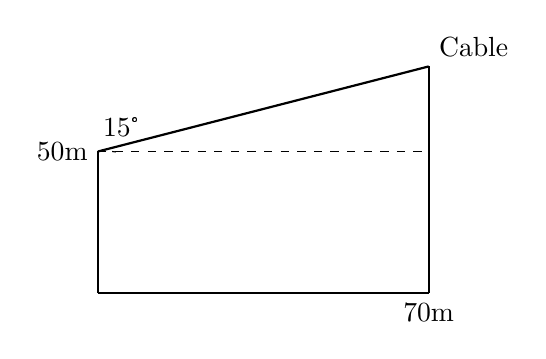
\begin{tikzpicture}[scale=0.6]
                % Shorter building
                \draw[thick] (0,0) -- (0,3) node[left] {50m};
                % Ground
                \draw[thick] (0,0) -- (7,0) node[below] {70m};
                % Taller building (unknown height)
                \draw[thick] (7,0) -- (7,4.8); % Placeholder height
                % Cable
                \draw[thick] (0,3) -- (7,4.8) node[above right] {Cable};

                % Horizontal line for angle reference
                \draw[dashed] (0,3) -- (7,3);
                % Angle of inclination
                \draw (0.3,3) arc (90:75:0.3); % Angle measured from the horizontal line
                \node[above] at (0.5,3.1) {15°};
            \end{tikzpicture}
        \end{columns}
    \end{tcolorbox}
\end{frame}
\end{document}